\subsection{Funzionamento del prisma di vetro}
Un prisma ottico di vetro è un solido trasparente delimitato da due superfici piane inclinate tra loro (le facce rifrattive) che formano un angolo al vertice $\alpha$. Quando un raggio di luce entra in un prisma, subisce due rifrazioni:

\begin{enumerate}
	\item \textbf{Prima rifrazione:} alla prima faccia di ingresso, quando il raggio passa dall'aria al vetro, deviando verso la normale alla superficie.
	\item \textbf{Seconda rifrazione:} alla seconda faccia, il raggio emerge dal prisma passando dal vetro all'aria, deviando lontano dalla normale.
\end{enumerate}

Queste due deviazioni cumulative producono uno scostamento del raggio emergente rispetto alla direzione originale del raggio incidente. L'effetto complessivo si chiama \textbf{deviazione angolare}.

\begin{figure}[H]
	\centering
	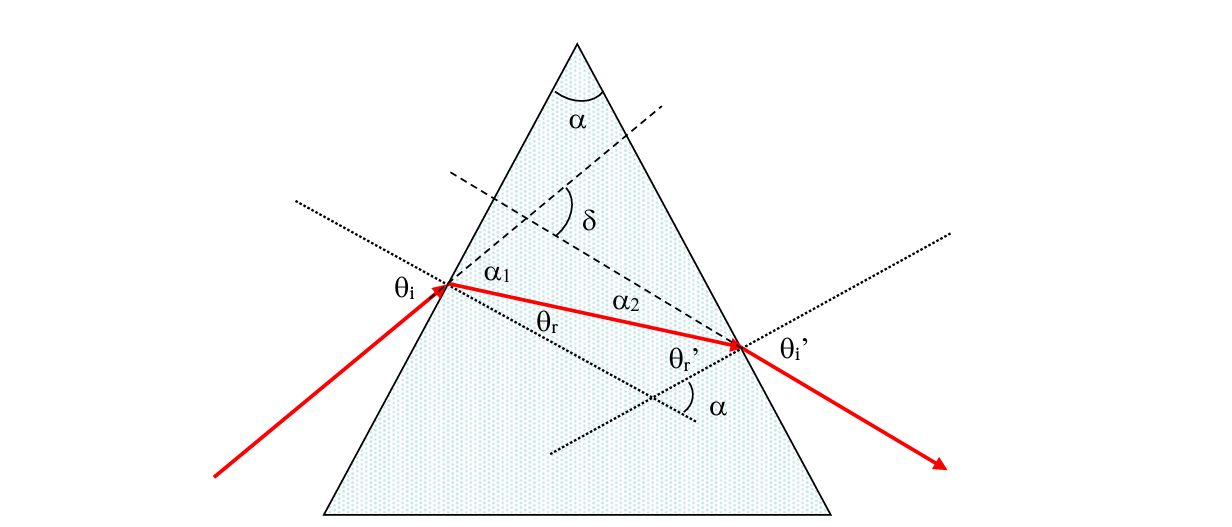
\includegraphics[width=0.75\textwidth]{./figures/prismateoria}
	\caption{Indichiamo: \\
		$\theta_i$ = angolo di incidenza sulla prima faccia (rispetto alla normale) \\
		$\theta_r$ = angolo di rifrazione dentro il prisma sulla prima faccia \\
		$\theta_r'$ = angolo interno di incidenza sulla seconda faccia \\
		$\theta_i'$ = angolo di rifrazione fuori dal prisma (angolo di uscita)}
\end{figure}

Applicando la \textbf{Legge di Snell} alla prima rifrazione:
\begin{equation}
	n_{aria}\sin(\theta_i)=n_{vetro}\sin(\theta_r)
\end{equation}
Poiché $n_aria \approx 1$, si può semplificare:
\begin{equation}
	\sin(\theta_i)=n\sin(\theta_r)
\end{equation}
Dopo il passaggio attraverso il prisma, usando la geometria interna si trova che:
\begin{equation}
	\theta_r'=\alpha-\theta_r
\end{equation}
Applicando ancora la Legge di Snell all'uscita:
\begin{equation}
	n_{vetro}\sin(\theta_r')=n_{aria}\sin(\theta_i') \rightarrow n=\frac{\sin(\theta_i')}{\sin(\theta_r')}
\end{equation}

La deviazione totale $\delta$ è data dalla differenza angolare tra il prolungamento del raggio incidente e il raggio emergente. La formula generale è data dalla Legge (1). Se si cambia lentamente l'angolo di incidenza, l'angolo di deviazione $\delta$ dapprima diminuisce, raggiunge un valore minimo, poi ricomincia ad aumentare. In corrispondenza della deviazione minima $\delta_{min}$ accade che il percorso della luce dentro il prisma è simmetrico: $\theta_i$ e $\theta_i'$ sono uguali, così come $\theta_r$ e $\theta_r'$. In questa situazione:
